\documentclass[9pt,twocolumn,twoside]{../../styles/osajnl}
\usepackage{fancyvrb}
\usepackage{comment}
\hypersetup{
	colorlinks=true,
	linkcolor=blue,
	filecolor=magenta,      
	urlcolor=blue,
}

\journal{i524} 

\title{Amazon Web Services Cloudmesh Extension}

\author[1]{Gregor von Laszewski}
\author[1]{Milind Suryawanshi}
\author[1]{Piyush Rai}

\affil[1]{School of Informatics and Computing, Bloomington, IN 47408, U.S.A.}


\dates{project-006, \today}

\ociscodes{Cloud, I524}

% replace this with your url in github/gitlab
\doi{Report:
	\url{https://github.com/cloudmesh/sp17-i524/blob/master/project/S17-IR-P006/report/report.pdf}\\
	Code: \url{https://github.com/cloudmesh/cloudmesh.aws}}


\begin{abstract}
	
Cloudmesh client provides and easy abstraction to gain access to hybrid
clouds from the commandline. In contrast to other systems it provides
a mechanism of adding plugins to the command. The command can not only
be used as a commandline tool, but as a shell. Due to the swift
developments in the area of cyber infrastructure such a convenient
plugin allows us to integrate easily new services easily. This work
uses our next generation cloudmesh shell and demonstrates the ease of
integrating Amazon Web Services services into it. Hence Cloudmesh
client can via other plugins achieve interoperability for virtual
machine management by providing plugins for OpenStack, Azure, Comet
Cloud Services and other frameworks including containers. Here we
focus on extensions to bring its capability to work with Amazon EC2
services. As our integration demonstrates how to leverage libcloud as a
backend, more than 30 other providers could easily be targeted.
 
\end{abstract}

\setboolean{displaycopyright}{true}

\begin{document}

\maketitle

\section{Introduction}


\TODO{Gregor: will include section about cloudmesh \cite{www-cloudmesh-client}}

Amazon provides a web service in a cloud (AWS) to deploy
virtual machines (VM) with numerous operating systems environment
available in different flavors. The images are called Amazon Machine
Image (AMI) and are available as pre-configured for different
applications. Once can also create his own custom environment
\cite{www-amazon-ec2}.

The Amazon EC2 drivers provides numerous functionalities to
authenticate into the AWS, list available configurations and create
and boot VMs. Many interfaces exist providing access to many different
frameworks and platforms. Being able to utilize access through Web
services allows developers to integrate AWS into their service
offerings. Within Indiana University we have provided for the last
seven years cloud services based on a variety of cloud services.
While observing the evolution and practical use of these services it
has become clear that in order to switch easily from one cloud to
another we need a uniform interfaces that provides the most elementary
service offerings of managing virtual machines. Our design offers tha
ability to switch easily between different cloud providers. Figure
\ref{F:switch} demonstrates this convenient feature. Here we define in
our cloudmesh client a cloud and set it to AWS, we than start a vm, we
can do the same for OpenStack as demonstrated. Important to note is
that all details of name assignment, flavor and image management, are
abstracted out, but can be controlled and are provided as part of an
easy to manage configuration framework. This has advantages for
university settings as we can distribute such configurations for
particular classes and customize the use for many hundrets of non
cloud experts. In fact using our abstractions allows non cloud experts
easily to use clouds. 

\begin{figure}[htb]
  \centering
  \begin{verbatim}
  set default cloud=aws
  vm boot
  set default cloud=openstack
  vm boot 
  \end{verbatim}
  \vspace{-2.0\baselineskip}
  \caption{cms aws image refresh}
  \label{fig:imagerefresh}
\end{figure}
		

\section{Design}

\subsection{Requirements}

\TODO{Requirements are missing}

\section{Implementation considerations}

The AWS client is based on cloudmesh.cmd5 \cite{www-cloudmesh-cmd5}
and cloudmesh.common \cite{www-cloudmesh-common}. It uses mongodb in
the back-end to store the cloud information such as list of available
images or instances running on the cloud. Requests library
\cite{www-python-requests} is used to connect to the back-end through
rest services. The rest service is deployed using cloudmesh REST
framework \cite{www-cloudmesh-rest}.

\TODO{Design Diagram is missing}
\begin{verbatim}
client -> rest (eve) -> database (nosql)
           ^ object definitions
\end{verbatim}

\section{Implementation}

\TODO{Some details about REST service and auto creation from
  examples. Gregor may have text.}


\section{Architecture}

The commands are implemented as methods of a class AwsCommand which is
based on PluginCommand from cloudmesh shell. Depending on the
arguments passed, corresponding routine is called from Aws client API
which acts as a wrapper around the libcloud EC2 drivers
\cite{www-libcloud-ec2} and is also responsible to connect with
back-end database apart from reading the configuration from yaml
file. The entire code is written in Python.

\subsection{Technologies Used}

To adhere to the principal of code reuse we are using a number of core
technologies that allow us to keep the overall developed new code
small. This includes leveraging our previous {\it cloudmesh} efforts, the
reuse of {\it mongodb} and the automatic creation of a REST service based
on example objects with {\it evengine}. Particularly the following
software components have been leveraged:

\begin{description}

\item [Libcloud EC2 driver \cite{??}:] The driver provides a number of functions
  for various functionalities such as listing the available nodes,
  generating a key pair and deploying a VM.

\item [MongoDb  \cite{??}:] MongoDB is an open source document store database. It's
  used by AWS client to store information about various VM
  configuration options available on the Amazon EC2 cloud. It's also
  used to store information regarding the VMs that are running on the
  cloud. The information in the database is refreshed whenever it's
  fetched from the cloud.

\item [Cloudmesh.common \cite{www-cloudmesh-common}:] A library of
  many commonly useful functions and classes shared among all
  cloudmesh projects.

\item [Cloudmesh.cmd5:] The cmd5 is a dynamically extensible CMD based
  command shell \cite{www-cloudmesh-cmd5}.

\item [Cloudmesh.evegenie \cite{www-cloudmesh-evengine}:] The schema for the collections are specified
  in json files which are then converted to Eve syntax using
  evegenie. It creates the configuration file for starting up the rest
  services using cloudmesh rest framework.
	 	
\item [Cloudmesh.rest \cite{www-cloudmesh-rest}:] The cloudmesh rest
  framework is used to deploy and start the mongodb and rest
  services. The schema for the objects to be stored in the database is
  collectively specified in json file called {\it all.json}. The
  schema defined in the file is closely associated with the code in
  awsclient.py which is responsible for fetching the information from
  cloud and passing it to mongodb through rest services. From our
  experience during the development of this project, we observed that
  rest services required the schema to be precise and didn't handle
  null values for collection fields. There's another file
  all.settings.py which contains the configuration information for
  rest services such as port mongodb is running on along with the
  database name. It contains the schema for the collections and the
  list of methods to be provided by the rest services. The database
  connectivity was initially developed using pymongo library. However,
  during the review it was suggested that the code based on pymongo is
  quite low level and does not have adequate security features. This
  led to the use of Pyhthon Requests library.
	
\end{description}

\section{Usage}

One needs to create an AWS account first to be able to access its
cloud. The instructions for it are available at
\cite{www-amazon-aws}. A pair of access key and secret keys are
required to be generated to authenticate into the cloud
\cite{www-amazon-key}. These keys are required to be kept
confidential. They are to be specified in a yaml configuration
file. Default vm image and flavor can also be specified in the
configuration file (see FIgure \ref{F:conf}). 

\begin{figure}[htb]
\begin{verbatim} 
cloudmesh:
  clouds:
    aws:
      credentials:
        EC2_ACCESS_KEY: 'ACCESS KEY'
        EC2_SECRET_KEY: 'SECRET KEY'
        . . .
    default:
      image: 'IMAGE ID'
      size: 'SIZE ID'
      location: 'LOCATION'
\end{verbatim}
\vspace{-1.0\baselineskip}
\caption{Configuration}\label{F:conf}
\end{figure}

The user need to ensure that the combination of image, size and
location is valid and that it's account has the required privileges
for it. The instructions for installation of AWS client can be found
at \cite{www-cloudmesh-aws}. Once, the client has been installed and
configurations settings enabled, the mongodb and the rest services to
access the database can be started by following command from the root
directory of the code:

\begin{verbatim}
    make rest
\end{verbatim}

The above services will be required by AWS client to store cloud
related information locally. The user can now execute the client
commands e.g.:

\begin{verbatim}
    cms aws flavor refresh
\end{verbatim}

This will fetch the list of image sizes available on Amazon EC2 cloud.

\section{AWS Commands}


\begin{table*}[p]
\caption{Cloudmesh AWS Commands}\label{T:aws-commands} 
\begin{center}
\begin{tabular}{p{2cm}p{10cm}p{5cm}}
  Function & Description & Command \\
  \hline
  Refresh &
            Whether to always fetch the information from the cloud
            over the network or display it from the local database when asked
            can be configured by setting the configuration variable {\it refresh} to
            either {\it on} or {\it off}. When the value is set to on, the information
            will always be fetched from the cloud.This functionality is
            implemented for only some of the commands as of now.
                         & \verb+aws refresh on+ \\
  \hline
  Image refresh&
                 The images available on the cloud could be listed
                 using this command. The database will also be updated with the newly
                 fetched list. The command may take up to minutes to run as the list
                 contains more than 24,000 images. 
    & \verb+aws image refresh+ \\
\hline
Image list & Depending on whether the value of {\it refresh} is
      set to {\it on} or {\it off}, the list is either fetched from the
      cloud or from the local database. &
    \verb+aws image list+\\
\hline	
Flavor refresh & This will list the different sizes of VMs
                   that are available on the cloud. The information is fetched from
                   the cloud and stored locally. & 
                                                   \verb+aws flavor refresh+ \\ 
\hline
Flavor list & The flavor list is either fetched from the
      cloud or from the local database depending on whether the
      value of {\it refresh} is set to {\it on} or {\it off}.
	
    \verb+aws flavor list+ \\
	
  \hline
  Start/Boot vm & It creates a new node instance and start that
                  node automatically. The required parameter is
                  \textit{IMAGE\_ID}. This command assumes user has created keypair
                  with name \textit{AWS1}. The default values; flavor and location are
                  taken from cloudmesh.yaml. Those values are required to be set
                  before executing this command. Once it has been created, it can be
                  seen using vm list.
                         & \verb+aws vm boot IMAGE_ID+ \\
  \hline
  Reboot vm & This command is used to reboot a running vm
              instance. The state of the node gets changed from RUNNING to
              REBOOTING while its restart. The rebooting time of node depends on
              the configuration the configuration that was selected while its
              creation. \textit{vm reboot} requires \textit{NODE\_UUID} of the
              node to be rebooted which can be retrieved using either \textit{vm
              list} or \textit{vm refresh}.
                         & \verb+aws vm reboot NODE_UUID+ \\
  \hline
  VM delete & It destroys the instance of a node and all the data
              associated with it including backup. It takes few seconds to
              terminated the instance. At first, the state of the node changes
              to \textit{TERMINATED} which can be observed using \textit{vm
              refresh} . The node gets removed from the list subsequently.
                         & \verb+aws vm delete UUID+ \\
  \hline
  VM list  & It lists out all the nodes along with their status as stored in the database.
                         & \verb+aws vm list+ \\
  \hline
  Keypair create & To create the node, one of the essential component is \textit{key pair}. Amazon EC2 uses public key of the user to encrypt the password and then recipient uses private key to decrypt it. These public and private keys are know as a \textit{key pair}. They are required to be given a name.
                         & \verb+aws keypair create NAME+ \\
  \hline
  Keypair delete & It allows user to delete a created \textit{key pair} which is no longer in use.
                         & \verb+aws keypair delete NAME+ \\
  \hline
  Keypair refresh & It refreshes the list of created \textit{key pairs} in the database and also displays it on the screen.
                         & \verb+aws keypair refresh+ \\
  \hline
  Keypairs list & It lists out all the \textit{key pairs} information stored locally in the database.
                         & \verb+aws keypair list+ \\
  \hline
  Keypair get & It returns the key pair object, which has the name of \textit{key pairs}, driver and hash key.
                         & \verb+aws keypair get NAME+ \\
  \hline
\end{tabular}
\end{center}
\end{table*}


\begin{table*}[htb]
\caption{Cloudmesh AWS Commands}\label{T:aws-commands} 
\begin{center}
\begin{tabular}{p{2cm}p{10cm}p{5cm}}
  Locations refresh & It will show all the available locations associated with Amazon EC2 account. For free tier, user will get two locations. More locations will be available in paid service. The database records are also updated with this command.
                         & \verb+aws location refresh+ \\
  \hline
  Locations list & It lists the locations information stored in the database.
                         & \verb+aws location list+ \\
  \hline
  Volume create & It creates the volume for vm. The size of volume is specified in GB, the default value is set to 1 GB. The maximum number of volumes that can be attached to a vm will depend on its operating system.
                         & \verb+aws volume create VOLUME_NAME+ \\
  \hline
  Volume refresh & This command shows the created volumes with the id, size and the driver name. It also updates the database.
                         & \verb+aws volume refresh+ \\
  \hline
  Volume list & This command displays the volume information stored in the database.
                         & \verb+aws volume list+ \\
  \hline
  Volume delete & User can delete the unwanted volumes using the \textit{VOLUME\_ID}.
                         & \verb+aws volume delete VOLUME_ID+ \\
\end{tabular}
\end{center}
\end{table*}




	
	
\begin{figure}[htb]
  \centering
  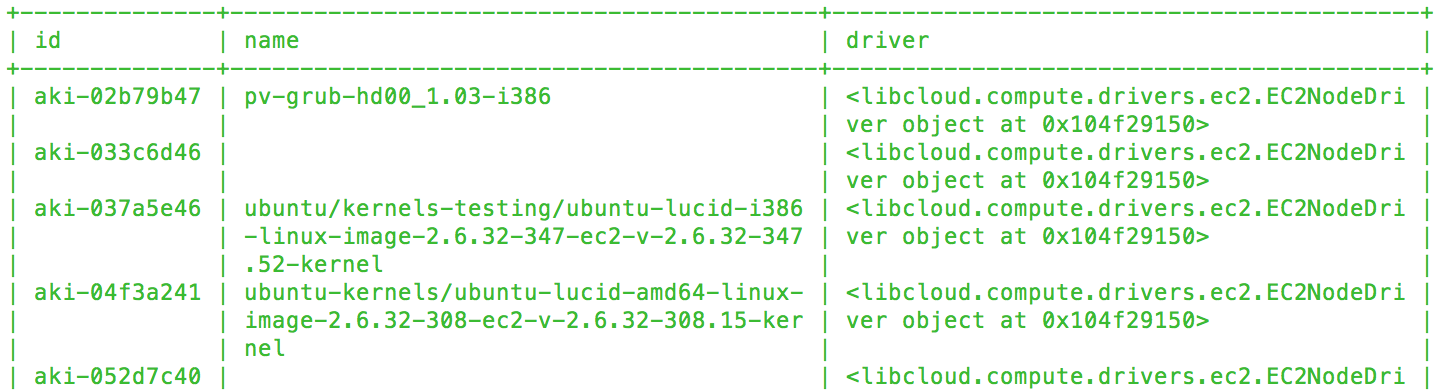
\includegraphics[width=\linewidth]{images/cms_aws_image_refresh.png}
  \vspace{-1.5\baselineskip}
  \caption{aws image refresh}
  \label{fig:imagerefresh}
%\end{figure}
~\newline
%\begin{figure}[h!]
  \centering
  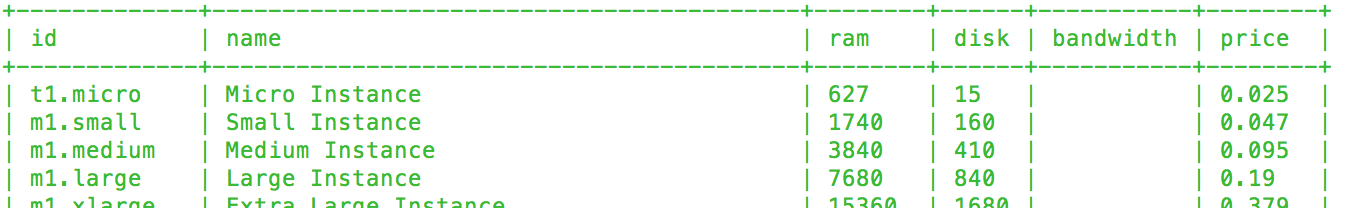
\includegraphics[width=\linewidth]{images/cms_aws_flavor_refresh.png}
  \vspace{-1.5\baselineskip}
  \caption{aws flavor refresh }
  \label{fig:flavorlist}
% \end{figure}
~\newline
% \begin{figure}[htb]
  \centering
  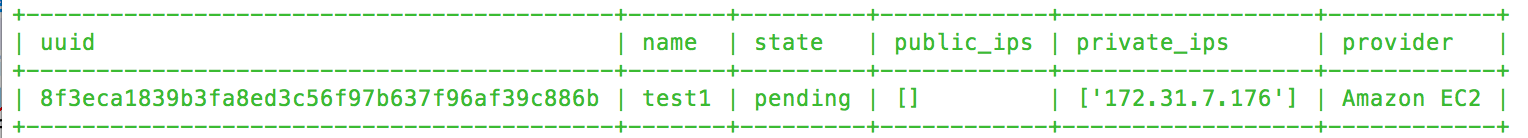
\includegraphics[width=\linewidth]{images/vm_boot_ami-0183d861.png}
  \vspace{-1.5\baselineskip}
  \caption{aws vm boot ami-0183d861 }
  \label{fig:vmboot}
% \end{figure}
~\newline
% \begin{figure}[htb]
  \centering
  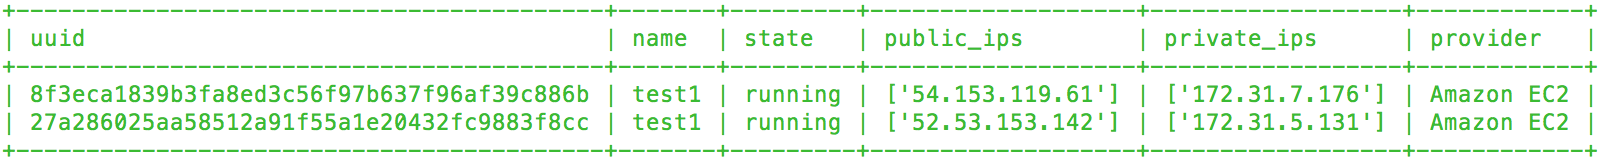
\includegraphics[width=\linewidth]{images/vm_list.png}
  \vspace{-1.5\baselineskip}
  \caption{aws vm list }
  \label{fig:vmlist}
% \end{figure}
~\newline
% \begin{figure}[h!]
  \centering
  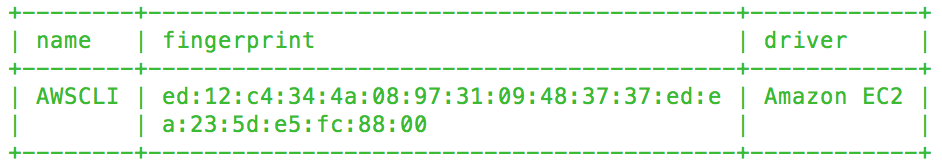
\includegraphics[width=\linewidth]{images/cms_aws_keypair_create.png}
  \vspace{-1.5\baselineskip}
  \caption{aws keypair create AWSCLI}
  \label{fig:keypaircreate}
% \end{figure}
~\newline
% \begin{figure}[h!]
  \centering
  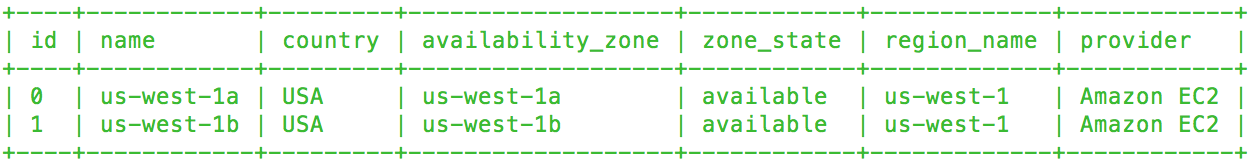
\includegraphics[width=\linewidth]{images/cms_aws_location_list.png}
  \vspace{-1.5\baselineskip}
  \caption{aws location refresh}
  \label{fig:locationlist}
%\end{figure}
~\newline
%\begin{figure}[htb]
  \centering
  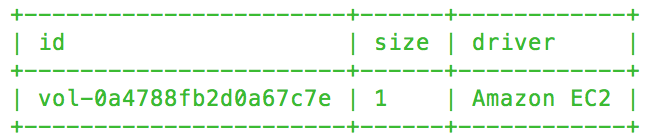
\includegraphics[width=0.5\linewidth]{images/cms_aws_volume_create_VOL_TEST_1.png}
  \vspace{-0.5\baselineskip}
  \caption{aws volume create VOL\_TEST\_1}
  \label{fig:createvolume}
%\end{figure}
~\newline
%\begin{figure}[htb]
  \centering
  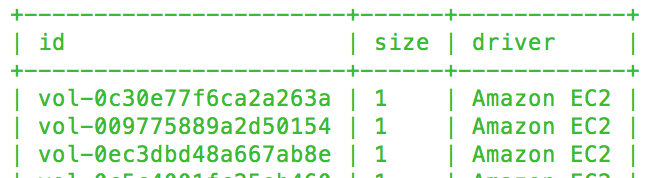
\includegraphics[width=0.5\linewidth]{images/cms_aws_volume_list.png}
  \caption{aws volume refresh}
  \label{fig:volumelist}
\end{figure}
    
\section{Benchmark}

\TODO{Benchmarks missing}

\section{Use Case: Create an AWS Node}
	The following are the pre-requisites to be able to create an EC2 node.

\subsection{Prerequisite}

\TODO{URLS IN REFRENCES}

\begin{enumerate}
	\item User should have a valid AWS account.
	\item \href{https://console.aws.amazon.com/iam/home?#/users}{Create a IAM}  user for which the access and secret key will have to be generated \cite{www-attach-policy}. The keys will ahve to added to the yaml cloudmesh configuraition file.
	
	\item The required permissions are needed to be granted to the user.
		\begin{enumerate}
			
			\item visit \href{https://console.aws.amazon.com/iam/home} {IAM home}
			\item select \textbf{policie}s in left hand menu
			\item create \textbf{administrator policy} from amazons existing policies
			\item select \textbf{administrator checkbox} and \textbf{attach} to your user
		\end{enumerate}
		
	\item Open the ../cloudmesh.yaml configuration file and update with EC2\_ACCESS\_KEY, EC2\_SECRET\_KEY, you just copied. Now set default flavor, image and location, as t2.micro, ami-0183d861 and us-west-1 respectively in same file.
	\item Mongodb server should be up and running (please refer section 2. Getting started)

\subsection{Create Node}

\begin{enumerate}
	\item Create keypair name using command
	
	\begin{verbatim}
	cms aws keypair create  AWS1
	\end{verbatim}
	
	It will create the \textit{keypair name}, it is essential to create the \textit{node}. To verify it, \textit{cms aws keypair list} command will list down all created \textit{keypairs} so far.
	
	\item Now create the node 
	
	\begin{verbatim}
	cms aws vm boot ami-0183d861
	\end{verbatim}
	
	Above command will create a node instance with the image of ami-0183d8661.

\end{enumerate}	
\end{enumerate}	
	

\begin{comment}
\section*{Acknowledgements}

Prof. Gregor von Laszewski originally suggested this project and
provided the objectives in simplistic form. He reviewd the code as it
was developed during the course of this project. His inputs helped us
to make the code more secure and efficient. He provided us with
different resources to look for help and overcome the challenges faced
during the course.
\end{comment}

% Bibliography

\bibliography{references}
 
\section*{Author Biographies}
\begingroup
\setlength\intextsep{0pt}
\begin{minipage}{1.0\columnwidth}
  \noindent
  {\bfseries Milind Suryawanshi} received his BE (Electronics and
  Telecommunication) in 2010 from The University of Pune. His research
  interests include Big Data analytics for intelligence and research.
\end{minipage}
\begin{minipage}{1.0\columnwidth} 
  \noindent
  {\bfseries Piyush Rai} received his BE (Computer) in 2011 from The
  University of Pune. His research interests also include Big Data
  analytics for military intelligence and frinancial markets.
\end{minipage}
\begin{minipage}{1.0\columnwidth} 
  \noindent
  {\bfseries Gregor von Laszewski} has written more than 100
  publications in the are of Grid and Cloud computing. He obtained a
  Ph.D. from Syracuse University and has worked at Argonne National
  Laboratory. His team is providing with cloudmesh a client interface
  to XSEDE SDSC comet virtual clusters.
\end{minipage}

\endgroup


\end{document}
